\documentclass[a4paper,12pt]{article}
\usepackage[osf]{mathpazo}
\usepackage{ms}
\usepackage[numbers, sort&compress]{natbib}
\usepackage{lineno}
\usepackage{graphicx}
\usepackage{caption}
\modulolinenumbers[5]
\linenumbers

\pdfminorversion=3

\makeatletter
\renewcommand{\@biblabel}[1]{\quad#1.}
\makeatother

\title{Common phylogenetic trait models are widely inadequate}
\author{
Matthew W. Pennell$^{1, *}$, Richard G. FitzJohn$^2$,\\
William K. Cornwell$^{3}$ \& Luke J. Harmon$^{1,4}$
}

\date{}
\affiliation{
 $^{1}$ Department of Biological Sciences \& Institute for Bioinformatics and Evolutionary Studies, University of Idaho, Moscow, ID 83844, U.S.A.\\ 
 $^{*}$ Email for correspondence: \texttt{mwpennell@gmail.com}\\
 $^{2}$ Department of Biological Sciences, Macquarie University, Sydney, NSW 2109, Australia;
\texttt{rich.fitzjohn@gmail.com}\\
 $^{3}$ School of Biological, Earth and Environmental Sciences, University of New South Wales, Sydney, NSW 2052, Australia; \texttt{w.cornwell@unsw.edu.au}\\
 $^{4}$ \texttt{lukeh@uidaho.edu}
}

\runninghead{are macroevolutionary models adequate?}
\keywords{comparative methods, model adequacy, independent contrasts, Brownian motion}


\begin{document}

\mstitlepage
\parindent=1.5em
\addtolength{\parskip}{.3em}
\vfill

\singlespacing
\section{Abstract}
Phylogenetic comparative methods (PCMs) provide a unique historical perspective on evolutionary questions and are being now used in an increasingly wide variety of fields to test hypotheses with interspecific data. As modern PCMs are almost exclusively statistical, inferences made from them also depend on a model describing the evolution of the trait along the phylogeny. The choice of the model is crucial --- the model needs to provide a good explanation for the data if inferences are to be reliable. To date, researchers have primarily assessed the explanatory power of the model by comparing the relative fit of a model to a small set of alternatives. A broader question is whether a model is a good absolute fit to the data; however, we currently have no way to address this. We address two outstanding problems in comparative biology. First, we develop a general framework, based on Felsenstein's independent contrasts method, for assessing the absolute fit, or adequacy, of phylogenetic trait models. This approach can be applied to arbitrarily complex models of quantiative trait evolution. Second, we ask whether the simple models commonly used in PCMs are adequate descriptiors of the macroevolutionary dynmaics of real comparative data. We fit three common models of trait evolution to 337 comparative datasets covering 3 key Angiosperm functional traits (specific leaf area, seed mass and leaf nitrogen), compiled from the literature. We find that these models are very poor models for trait evolution. This was true across many clades at many different scales though their adequacy was much worse at larger scales. Furthermore, the relative support for a model, as evaluated using conventional model selection criteria, had very little to do with absolute model adequacy. Our results raise very serious concerns about current practices in comparative biology. We argue that assessing model adequacy should be a routine component of phylogenetic comparative studies.

\vfill

\newpage



\begin{quotation}
\noindent There are known knowns; there are things we know we know. There are known unknowns; that is to say, there are things that we now know we don't know. But there are also unknown unknowns --- there are things we do not know we don't know.

---Fmr. U.S. Secretary of Defense Donald Rumsfeld
\end{quotation}

\section{Introduction}
Nothing in biology makes sense except in light of phylogeny. Phylogenetic trees and phylogenetic thinking are ubiquitous in modern biology; ecologists, geneticists, paleontologists and anthropologists now widely recognize that a historical perspective can provide novel insights into evolutionary questions. 

This interest in phylogenetic biology has risen in lockstep with developments in phylogenetic comparative methods (PCMs; reviewed in \citep{PennellHarmon}). Modern PCMs are almost exclusively model--based, meaning inferences are contigent on both the phylogenetic tree and the chosen probabilistic model. Selecting a good model is therefore essential for making robust inferences. Model choice should be guided by two considerations. First, does the model capture the processes relevant to the question \citep{HansenOrzack2005, Hansen2012, PennellPE}? Second, does the model provide a good statistical explanation for the data? Though there is interplay between these two questions \citep{Hansen2012}, the latter is the focus of this paper. In phylogenetic comparative biology, this question has been addressed by comparing the relative fit of a number of models and selecting the best one for inference \citep{Mooers1999, Harmon2010, Hunt2012}. 

But the relative support for a model is only a partial answer to the question of whether it is a good explanation for the data. We also must consider whether the model is a good fit, or adequate, on its own terms. The best of a poor set of models is still a poor model. Assessing model adequacy is a routine step in many statistical applications, especially Bayesian statistics \citep{Gelmanbook}. Failure to check model adequacy can potentially result in erroneous inferences. A classic example of this in molecular systematics is the disputed phylogenetic relationships of rodents. A number of early molecular phylogenetic studies reported evidence that ``strongly contradict[ed]'' the traditional hypothesis that the order Rodentia is a monophyletic group \citep{Graur1991, DErchia1996}. Sullivan and Swofford \citep{SullivanSwofford} demonstrated that these conclusions were misleading, and resulted entirely from using models of molecular evolution that did not adequately accomodate  heterogeneity in rates of evolution across sites. There are many similar case--studies throughout and outside of evolutionary biology.

Many models for describing the evolution of phenotypic traits along a phylogeny have been developed, as well as sophisticated machinery for fitting them to data (e.g., \citep{Felsenstein1985, Hansen1997, Pagel1999, Blomberg2003, ButlerKing2004, Omeara2006, Eastman2011, Beaulieu2012, SlaterMEE, UyedaBayou}). Using these models, researchers from across biological disciplines have made exciting discoveries that would not have been possible without a phylogenetic perspective. However, it is disconcerting that we generally have no idea if the models used in PCMs are adequate; there are no general procedures that can be used to assess the adequacy of the models most often used in comparative biology. Even more troubling is that model adequacy is rarely ever considered when PCMs are applied. To borrow Rumsfeld's taxonomy, model adequacy has largely been an ``unknown unknown'' in PCMs.

In this paper we seek to (at least somewhat) rectify this situation. We address two major outstanding problems in comparative biology. First, we develop a general framework for assessing the adequacy of phylogenetic models of trait change, specifically those for quantitative characters. Second, we assess the adequacy of commonly used models of trait evolution, using a recently published mega--phylogeny of Angiosperms (flowering plants) \citep{Zanne2013} and data on three important functional traits --- specific leaf area, seed mass, and leaf nitrogen content --- compiled from the literature. We did this to ask whether the simple models used in comparative biology provide a reasonable descriptor of the macroevolutionary dynamics of real trait data, and at what phylogenetic scale are they appropriate.

\section{A general framework for assessing model adequacy}
The basic concept of our approach is as follows. We have a phylogenetic tree consisting of $n$ lineages. We have data on the the trait values observed at each tip $X$ ($X= X_1, X_2, \ldots, X_n$). In order to make inferences from the distribution of traits at the tips, we fit a model $\mathcal{M}$, describing the evolution of the trait along the phylogeny, and estimate a set of parameters $\Theta_{\mathcal{M}}$. Most analyses using comparative data aim to answer one of the following questions: what $\Theta_{\mathcal{M}}$  maximizes the probability of observing $X|\mathcal{M}$?; what is the posterior distribution of $\Theta_{\mathcal{M}}|X, \mathcal{M}$?; or, does $\mathcal{M}_1$ explain the data better than $\mathcal{M}_0$? Our approach is conceptually distinct in that we want to ask, how likely is it that $\mathcal{M}$ would produce a dataset similar to $X$ if we re--ran evolution?

We have developed two separate ways to ask this question --- one frequentist, the other Bayesian. While these approaches are philosophically different from one another, in practice, they are very similar. In a frequentist paradigm, we can assess model adequacy by performing parametric bootstrapping. We estimate $\Theta_{\mathcal{M}}$ using maximum likelihood, restricted maximum likelihood, least--squares, etc. We then simulate new datasets $Y$ by evolving a trait along the phylogeny according to $\mathcal{M},\Theta_{\mathcal{M}}$. We can then compare $X$ and $Y$. However, in order to make any sort of comparison, we must first summarize $X$ and $Y$ using a meaningful summary statistic or a set of summary statistics $\mathcal{S}$. If the elements of $\mathcal{S}_X$ are in the tails of the corresponding distribution $\mathcal{S}_Y$, then, we can conclude that the model is not a good explanation for $X$. Parametric bootstrapping is likely familiar to phylogenetic biologists in the form of the Goldman--Cox test \citep{Goldman} for the adequacy of sequence evolution models.

Alternatively, one may adopt a Bayesian perspective and estimate the posterior distribution $\mathbb{P}(\Theta_{\mathcal{M}}|X,\mathcal{M})$ using Bayes theorem
\begin{equation}
\mathbb{P}(\Theta_{\mathcal{M}}|X,\mathcal{M}) = \frac{\mathbb{P}(X|\Theta_{\mathcal{M}}, \mathcal{M})\mathbb{P}(\Theta_\mathcal{M}, \mathcal{M})}{\mathbb{P}(X|\mathcal{M})}
\end{equation}
often (such as for models used in comparative biology) using Markov chain Monte Carlo (MCMC) machinery. To assess the adequacy of the model we perform posterior predictive simulations \citep{Rubin1984, Gelman1996}. The posterior predictive distribution is defined as
\begin{equation}
\mathbb{P}(Y|X,\mathcal{M}) = \int \mathbb{P}(Y|\Theta_{\mathcal{M}}, \mathcal{M})\mathbb{P}(\Theta_{\mathcal{M}}|X,\mathcal{M})d\Theta_{\mathcal{M}}.
\end{equation}
where $\mathbb{P}(Y|X,\mathcal{M})$ is the probability of a new dataset $Y$ given $X$ and $\mathcal{M}$. We obtain this distribution by drawing repeated samples from $\mathbb{P}(\Theta_{\mathcal{M}}|X,\mathcal{M})$ and simulating datasets from the sampled parameters. We can compute the summary statistics $\mathcal{S}_X$ over the distribution of $\Theta_{\mathcal{M}}|X,\mathcal{M}$ and $\mathcal{S}_Y$ over $Y|\mathcal{M},X$ and compare the $\mathcal{S}_X$ and $\mathcal{S}_Y$. Posterior predictive simulation appraoches have also been developed for molecular phylogenetics \citep{Bollback2002, Reid2013, Lewis2013, Brown2013} but have unfortunately not been widely adopted \citep{Brown2013}.


\subsection{Summary statistics}
As stated above, in order to compare the observed data $X$ with the data simulated under the fitted model $Y$ we need some way of summarizing the observations to make meaningful comparisons. 
In our approach we calculate a set of summary statistics on a set of contrasts (\textit{sensu} Felsenstein \citep{Felsenstein1985}) computed at each node, rather than on the data itself. (We refer readers to \citep{Felsenstein1985, Rohlf2001, Blomberg2012}, for details on how contrasts are calculated.) Contrasts are a natural way of summarizing phylogenetically structured quantiative data with very little loss of information. Importantly, under Brownian motion (BM) the contrasts will be independent and identically distributed (i.i.d.) $\sim \mathcal{N}(0, \sigma)$, where $\sigma^2$ is the BM rate parameter \citep{Felsenstein1985}. The trait data at the tips can only be i.i.d. if there is no phylogenetic signal in the data. 

We have chosen a set of six summary statistics $\mathcal{S}$ to compute on the contrasts of both our observed data and our simulated data.

\begin{enumerate}
\item[$M_{PIC}$] The mean of the squared contrasts. This is equivalent to the restricted maximum likelihood (REML) estimator of the Brownian motion rate parameter $\sigma^2$ \citep{Garland1992, Rohlf2001}. $\mathcal{S}_1$ is a metric of overall rate.

\item[$V_{PIC}$] The coefficient of variation for the absolute value of the contrasts. If $V_{PIC}$ calculated from the observed contrasts is greater than that calculated from the simulated contrasts, it suggests that we are not properly accounting for rate heterogeneity across the phylogeny. If $V_{PIC}$ from the observed is smaller, it suggests that contrasts are more even than the model assumes. We use the coefficient of variation rather than the variance because the mean and variance of contrasts are tightly linked.

\item[$S_{VAR}$] The slope resulting from fitting a linear model to the absolute value of the contrasts vs. their expected variances. Each (standardized) contrast has an expected variance proportional to the sum of the branch lengths connecting the node at which it is computed to its daughter lineages  \citep{Felsenstein1985}. Under a model of BM, we expect no relationship between the contrasts and their variances. We use $\mathcal{S}_3$ to test if contrasts are larger or smaller than we expect based on their branch lengths. If, for example, more evolution occured per unit time on short branches than long branches, we would observe a negative slope.

\item[$S_{ANC}$] The slope resulting from fitting a linear model to the absolute value of the contrasts vs. the inferred ancestral state at the corresponding node. We estimated the ancestral state using the least--squares method suggested by Felsenstein \citep{Felsenstein1985} for the calculation of contrasts. We note that this is not technically an ancestral state reconstruction (see \citep{Felsenstein1985}); it is more properly thought of as a weighted average value for each node. We used this statistic to evaluate whether there is variation in rates relative to the trait value (e.g., do larger organisms evolve proportionally faster than smaller ones?)

\item[$S_{HGT}$] The slope resulting from fitting a linear model between the absolute value of the contrasts and the height of the node at which they are inferred measured from the root, with the node height as the independent variable. This is used to capture variation relative to time. It is alternatively known as the ``node--height test'' \citep{FreckletonHarvey2006, SlaterPennell} and used for detecting early bursts of trait evolution during adaptive radiations. 

\item[$D_{KS}$] The D--statistic obtained from Kolmolgorov--Smirnov test from comparing the distribution of contrasts to that of a normal distribution with mean 0 and standard deviation equal to the root of the mean of squared contrasts (the expected distribution of the contrasts under BM; see \citep{Felsenstein1985, Rohlf2001}). We chose this to capture deviations from normality. For example, if traits evolved via a ``jump--diffusion'' type process \citep{Landis2012}, in which there were occasional large ``jumps'' in phenotypic space \citep{PennellPE}, the tip data would no longer be multivariate normal owing to a few contrasts throughout the tree being much larger than the rest; i.e., the distribution of contrasts would have heavy tails. 

\end{enumerate}

We have chosen these six summary statistics because they capture a range of dimensions of variability wherein the model may not be adequate. However, they are certainly not exhaustive. One could, for instance, calculate the median of the squared contrasts, the skew of the distribution of contrasts, etc. If the generating model was known, we could use established procedures for selecting a set of sufficient (or, approximately sufficient \citep{MajoramJoyce}) summary statistics for that model. However, the aim of our approach is assess the fit of a proposed model without reference to a true model. The choice of what summary statistics to use is ultimately one of balancing statistical intuition and computational effort. Unfortunately, there is no good statistical theory to guide us as to which summary statistics to use and how many are enough \citep{Gelmanbook}. Our chosen statistics capture a wide variety of model misspecifications but this does not mean that they will necessarily capture every type of model misspecification; researchers interested in specific questions are encouraged to explore alternate sets of summary statistics. 

\subsection*{Beyond Brownian motion}

All of the summary statistics essentially test the assumption that the contrasts are i.i.d. $\sim\mathcal{N}(0, \sigma)$, which is expected under BM. We can reject a BM model if this condition does not hold. Our summary statistics $S_{VAR}$, $S_{ANC}$, and $S_{HGT}$ have been used previously in the literature with this justification \citep{Garland1992, Garland1993,  Diaz1996}. However, if we propose a different model for the evolution of the trait, such as an Ornstein--Uhlenbeck (OU; \citep{Hansen1997}) or a multi--rate BM model \citep{Omeara2006}, then the expected distribution of the contrasts is different. The expected distribution of contrasts under most other (i.e., non--BM) models of trait evolution is not formally characterized and even if it was, this would necessitate a specific set of summary statistics for every model proposed.

Our solution to this problem is to create what we term a ``unit tree''. A unit tree is defined as a phylogeny which has branch lengths in units of expected (standardized) variance. We can rescale a phylogeny with branch lengths in time units to a unit tree using the parameters of any quantitative trait model, as long as the data at the tips is assumed to come from a multivariate normal distribution (see Box 1 for details). This applies to nearly all models currently used in comparative biology \citep{Omeara2012}. If the fitted model is adequate, the trait data at the tips of the unit tree will have the same distribution as data generated under a BM process with a rate of 1 and the contrasts will be $\sim \mathcal{N}(0,1)$ (hence the name, unit tree). Creating the unit tree from the estimated model parameters prior to computing the contrasts generalizes the summary statistics to most models of trait evolution.

Calculating the contrasts on the unit tree also means that rather than simulate trait evolution under the model, we can simulate many datasets under a BM process ($\sigma^2 =$ 1). The distribution of summary statistics calculated on these simulated data sets can then be compared to the summary statistics from the observed data. We summarize the entire approach in Figure \ref{fig:flowchart}.

\begin{center}
\textit{[Box 1 around here]}
\end{center}

\section{The adequacy of models for the evolution of plant functional traits}

We used the approach we developed to address an outstanding question in comparative biology: how well do commonly used models explain the evolution of traits along a phylogeny and when are more complex models required. We addressed this question by studying Angiosperm functional traits using a recently published a megaphylogeny of containing 31,749 species of seed plants \citep{Zanne2013}. This dataset is exceptional in terms of scope and allowed us to evaluate the adequacy of models through time and across many groups.  

We compiled data on three traits from the literature: specific leaf area (SLA), defined as fresh area/dry mass; seed mass; and leaf nitrogen content (\% mass) (see Methods for details on datasets). SLA and leaf nitrogen content are important and widely measured components of the leaf economic spectrum, which relates to a plant's ecological strategy (i.e., how it balances photosynthetic capabilities and hydrodynamic cycling) \citep{Westoby2002, Wright2004}. Seed mass is an important proxy for many life--history traits \citep{Westoby2002, Moles2005}. Understanding the macroevolutionary patterns of these three traits can provide key insights into the evolutionary processes that have shaped much of plant diversity \citep{ksi}.  

We  matched these data to the phylogeny and then
%% Number of clades -- 337
pulled out 337 subclades, extracting named (family and orders) and unnamed clades taken from time--slices across the tree. Following Harmon et al. \citep{Harmon2010}, we fit three simple models of trait evolution to each subclade in the dataset: 1) BM, which can be associated with genetic drift \citep{Lande1976, Felsenstein1988, Lynch1990, HansenMartins1996}, randomly--varying selection \citep{Felsenstein1973}, or the summation of many independent processes over macroevolutionary time \citep{HansenMartins1996, Uyeda2011, PennellPE}; 2) single optimum OU, which is often assumed to represent stabilizing selection (following Lande \citep{Lande1976}), though we think a more meaningful interpretation is that it represents an ``adaptive zone'' \citep{Hansen2012book, PennellHarmon}; and 3) EB, which was developed as a mathematical represenation of a niche--filling process during an adaptive radiation \citep{Harmon2010, SlaterPennell}. We evaluated the relative support for each of the three models using conventional model selection techniques and then assessed the adequacy of the models using our procedure. (See Methods section for further details.) 


\subsection{A case study: seed size evolution in the Meliaceae and Fagaceae }
As an illustration of our approach, we present a case study examining seed size evolution in two tree families, the Meliaceae (the mahogany family) and Fagaceae (which contains oaks, chestnuts and beech trees). The trait data and phylogeny for both groups are subsets of the larger dataset used in the analysis (see above, Methods). Superficially, these datasets are quite similar. Both are of similar size (Meliaceae: 44 species in dataset; Fagaceae: 70 species) and are ecologically comparable. As stated above, we fit three simple models of trait evolution (BM, OU, EB) to both datasets and computed AIC weights \citep{aicweight} for the three models. For both datasets, an OU model was overwhelmingly supported (AICw $>$ 0.97 for both groups). Using the conventional model selection approach commonly used in comparative biology, we might conclude that similar evolutionary processes are important in these two clades of trees.

%% Meliaceae seedmass p-values (OU)
%%     m.pic     v.pic     s.var     s.anc     s.hgt      d.ks
%% 0.4535465 0.4895105 0.6233766 0.4655345 0.1478521 0.6233766
%%
%% Fagaceae seedmass p-values (OU)
%%     m.pic     v.pic     s.var     s.anc     s.hgt      d.ks
%% 0.001998002 0.5914086 0.2077922 0.3636364 0.8211788 0.9170829
Examining model adequacy provides an alternative perspective. We took the MLE of the parameters from the OU models for each dataset, constructed a unit tree based on those parameters. We calculated our six summary statistics on the contrasts of the data, then simulated 1000 BM datasets on the unit tree and calculated the summary statistics on the contrasts of each simulated dataset. The results from the analyses of model adequacy are shown in Figure \ref{fig:two-clades}. For seed size evolution in Meliaceae, the OU model selected by AIC was an adequate model; all six observed summary statistics were in the middle of the distribution of simulated summary statistics ($M_{PIC}: p=0.453$, $V_{PIC}: p=0.490$, $S_{VAR}: p=0.623$, $S_{ANC}:p=0.466$, $S_{HGT}: p=0.148$, $D_{KS}: p=0.623$). For the Fagaceae, the story is different. The OU model was revealed to be inadequate by $M_{PIC}$ ($p=0.002$); the rest of the observed summary statistics did not differ significantly from the simulated summary statistics ($V_{PIC}:p=0.591, S_{VAR}: p=0.207$, $S_{ANC}:p=0.364$, $S_{HGT}: p=0.821$, $D_{KS}: p=0.917$). $M_{PIC}$, the REML estimate of $\sigma^2$ was significantly lower than the expectation based on the model, suggesting that the process of evolution that gave rise to this data is more complex that that captured by a simple OU process. This example serves to illustrate the distinction between the conventional approach to model selection in PCMs and model adequacy. Selecting amongst a limited pool of models does not give a complete picture of whether a model is appopriate. We will return to this case study in this discussion.


\section{Empirical Results}

All analyses were performed using both likelihood and Bayesian methods (see Data and Methods). For the sake of clarity, we present only the results from likelihood analyses here. Results from Bayesian inference were qualitatively similar and are presented in full in the Supplementary Material. Across the 337 subclades, we found widespread support for OU
%% n. clades OU best supported model: 236
models. For 236 of clades, OU had the highest AIC weight.
%% n. clades OU supported with 100% aicw: 25
%% n. clades OU supported with >75% aicw: 186
OU had $\sim$100\% of the AIC weight in 25 clades and $>$75\% of the weight in 186 clades (Figure \ref{fig:aic-support}). Similar to the analysis of Harmon et al. \citep{Harmon2010} we found very little support for EB models (only 6 clades supported EB with $>$75\% of the AIC weight), suggesting that ``early bursts'' of trait evolution may indeed be rare in comparative data (but see \citep{SlaterPennell}). Larger clades were
%% n. clades with more than 100 taxa: 101
%% of these, how many had a single model with >90% support: 58
likely to have high support for a single model (of the 101 clades consisting of more than 100 taxa, 58 had had $>$90 of the AIC weight on a single model),
%% of these 58, how many were OU: 56
and that was overwhelmingly likely to be an OU model (56/58 clades). 

We limit our analyses of model adequacy to only the most highly supported model in the candidate set, as supported by AIC. We did this to present a best--case scenario; if a model had very little relative support, it would be unremarkable if it also had poor adequacy (but see \citep{Ripplinger2010}). Even considering only the best model, the models, in general, had strikingly poor adequacy (Figure \ref{fig:pvalues}). 
%% SLA data for 72 clades
%% rejected by at least one ss: 72
%% rejected by at least two ss: 35
%% rejected by at least three ss: 15
Of the 72 comparative datasets of SLA, all 72 rejected the best model by at least one summary statistic (using a cut--off of $p=$0.05), 35 by at least two, and 15 by three or more. 
%% Seed mass data for 226 clades
%% rejected by at least one ss: 185
%% rejected by at least two ss: 120
%% rejected by at least three ss: 64
Results were similar in the seed mass data (of the 226 seed mass datasets, 185 were rejected by at least one summary statistic, 120 by at least two and 64 by three or more) and leaf nitrogen content 
%% Leaf nitrogen data for 39 clades
%% rejected by at least one ss: 39
%% rejected by at least two ss: 21
%% rejected by at least three ss: 11
(of the 39 datasets, all 39 could be rejected by at least one, 21 by at least two, and 11 by three or more summary statistic). 
%% statistics which were most often violated
%% rejected by m.pic: 250
%% rejected by v.pic: 174
%% rejected by s.var: 60
%% rejected by s.anc: 67
%% rejected by s.hgt: 35
%% rejected by d.ks: 61
Some summary statistics were much more likely to detect model violations than others. The best model was rejected by $M_{PIC}$ in 250 datasets and by $V_{PIC}$ in 174; the frequency of rejection is substantially lower by the other summary statistics ($S_{VAR}$: 60, $S_{ANC}$: 67, $S_{HGT}$: 35, $D_{KS}$: 61). 
%% The number of datasets which were adequately modeled: 41
Across all 337 datasets, only 41 are adequately modeled by either BM, OU or EB; all of these are seed mass datasets. This is extremely worrisome as these are some of the most commonly used models in comparative biology. 

As the subclades are not independent (overlapping sets of taxa are present in family, order and time--slice phylogenies), conventional statistics, such as linear regression, are not straightforward to apply across datasets. Nonetheless, the trend is clear: the larger the phylogeny, the more likely OU is to be highly supported and the more likely the model is to be inadequate. There is a strong relationship between the size of a subclade and the overall distance between observed and simulated summary statistics (Figure \ref{size:adequacy}). This is not simply an artifact of conducting the analyses using a larger number of contrasts for the summary statistics --- if the model was adequate at all scales, there would be no relationship between the Mahalanobis distance and the size of the phylogeny. There appears to be a much weaker relationship between clade age and model adequacy (Supplemental Figure xx).

\section{Discussion}

The distinction between relative and absolute fit is an important one. A model may provide the the best explanation for a dataset compared to a few other models but still be a very poor explanation on its own terms. In our analyses of the evolution of three key Angiosperm functional traits, the fact that a model (most often, OU) was highly supported relative to the others, in many cases had little to do with the model's absolute explanatory power. Overall, the adequacy of the three simple, but commonly used, models of trait evolution was woefully poor (Figure \ref{fig-pvalues}). Perhaps surprisingly, this was true at across all scales, though models were increasingly inadequate at larger scales (Figure \ref{fig:size-adequacy}). Our results raise serious concerns about current practices in comparative biology. Relying on a single model (such as BM), or even the best among a small subset of models, for inference has the potential to greatly mislead inferences about the processes that have driven the evolution of traits at phylogenetic scales.

Of course, we are not the first to point this out. Many researchers have expressed concern that the models used in comparative biology are often inappropriate, for either biological or statistical reasons \citep{Felsenstein1985, Felsenstein1988, HarveyPagel1991, Garland1992, Pagel1993, Diaz1996, HansenMartins1996, Price1997, Garland1999, GarlandIves2000, HansenOrzack2005, Hansen2012, Felsenstein2012, Boettiger2012, SlaterPennell}; indeed, many of these issues were raised in the early days of the field. The contribution of this our paper to this discussion is that the development of a general approach for empirically evaluating the adequacy of arbitrarily complex models of trait evolution. We demonstrate the concerns about model inadequacy are not just theoretical but have real implications for real data.

The 337 comparative datasets we analyzed varied tremendously in terms of traits, size, age and placement in the Angiosperm phylogeny. Nonetheless, several general patterns emerge. An OU model, was by and large, the most supported of the three we examined. In an analysis of 67 comparative datasets consisting of size and shape data from a variety of animal taxa, Harmon et al. \citep{Harmon2010} also found substantial support for OU models, though for their datasets, BM was more commonly chosen by AIC (we note, however, that many of their datasets were quite small; see \citep{SlaterPennell}). Since their paper, a number of studies conducted in a diverse array of groups have also found OU models to be preferred over BM models (e.g., \citep{Burbrink2012, Wiens2013, Lopez2013}). Various evolutionary explanations have been proposed to explain these results \citep{HansenMartins1996, ButlerKing2004, Hansen2012book, PennellHarmon}. Our results suggest a statistical explanation for the widespread support of OU models. OU models predict higher variance near the tips of the phylogeny (i.e., between closely related taxa) than do BM or EB models (see Figure 1 in \citep{Harmon2010}). Heterogeneous evolutionary processes, phylogenetic mis--estimation (see below) and measurement error \citep{Houle2011, Hansen2012} could all produce such a pattern, even though these have nothing to do with the interpretations that have been put forth for OU models. In light of our results from model adequacy, it is likely that OU is widely supported simply because it is able to accomodate more ``slop'' than the other models.

This explanation is further supported by the how the observed summary statistics deviate from the simulated summary statistics. As stated above, model violations were most frequently detected by the global rate estimate $M_{PIC}$ (the best supported model using AIC  was rejected by $M_{PIC}$ in 250/337 datasets). These deviations were not random
%% in all 250 cases, observed mean less than mean of simulated means
 --- in all 250 of these cases, $M_{PIC}$ calculated from the observed contrasts was less than the mean of $M_{PIC}$ calculated from the contrasts of the data simulated on the unit tree. If the evolutionary process (or, alternatively, phylogenetic/measurement error) is heterogeneous across the tree, the lineages in some parts of the clade will be much more divergent than in others. The only way for the model to account for the highly divergent groups is to estimate a large $\sigma^2$ (and/or a small $\alpha$ parameter for the OU model). The unit tree formed by these parameter estimates will have long branches across the entire tree. In the less divergent parts of the tree, the contrasts calculated on this unit tree will be small, relative to what we expect under BM. So perhaps counter--intuitvely, when heterogeneity in processes across taxa cause the estimated global rates of divergence to be inflated, this will result in a lower value for $M_{PIC}$. For similar reasons, model inadequacy was also commonly detected with $V_{PIC}$, the coefficient of variation of the contrasts. For this summary statistic, the observed values tend to be \emph{larger} the the simulated values, though not as consistently as $M_{PIC}$ is smaller. 

Determining the underlying causes of differences in the adequacy of models across groups is both interesting and challenging. Returning to our case study fitting models to seed mass evolution in two clades of trees (see above, Figure \ref{fig:two-clades}), it is unclear why an OU model seems to describe the pattern of the trait in Meliaceae but not in Fagaceae (as detected by deviations in $M_{PIC}$). Both are woody lineages with large, usually vertebrate dispersed seeds \citep{Pannell1987, Manos2001}. One intriguing difference between the two clades is that some groups within Fagaceae are rapidly diversifying (e.g., within the genus \emph{Quercus}, see \citep{Simeone2013}). The same ecological processes may be implicated in driving rapid diversification and heterogeneous patterns of trait evolution across the group \citep{Schluter2000}, but we do not have any real evidence that this is the case. 

We also detected that these simple models often failed to capture other important types of heterogeneity --- variation with respect to branch lengths ($S_{VAR}$), trait values ($S_{ANC}$) and time ($S_{HGT}$). Additionally, a substantial number of datasets were not well--modeled by a multivariate normal distribution, suggesting that ``jumps'' in trait space may indeed be relatively common \citep{Landis2012, PennellPE}. The patterns of deviation between the observed and simulated summary statistics will often reflect interesting biology and can help guide researchers as to what additional processes are likely to be important in their group.

Several important caveats regarding this empirical test need to be stated. First, the models we fit were simplistic and we were certainly not so na\"{i}ve as to think they would be appropriate at very large scales; e.g., we knew that a single rate BM model was unrealistic for the evolution of seed mass across all Angiosperms \citep{Moles2005}. And there has been a great deal of progress towards more complex models of trait evolution that accomodate variation in models and rates across the tree (e.g., \citep{ButlerKing2004, Omeara2006, Eastman2011, Beaulieu2012, SlaterMEE, UyedaBayou}). We chose to analyze only the three models we did because: they are very commonly used; and doing so made results from one clade easy to compare with other clades in this and other studies. Second, the phylogeny we used is poorly resolved in some places, particularly, close to the tips. Many methodological shortcuts were necessary to construct a tree of this size and certainly, at least some of the poor performance of the models can be attributed to the inaccurate placement of taxa. However, though our dataset is exceptionally large, comparative analyses are increasingly being performed on very large phylogenies or subclades extracted from them, \citep{Coopermammal, Jetz2012, Rabosky2013, PyronBurbrink2013, ksi}. While the results of our analysis are striking, their generality will only be apparent once our approach has been applied to modeling fitting in many different comparative studies.

We are not advocating in this paper that the $p$--values obtained from simulations be used as a means of model selection; rather, we view model checking as a step that should follow model choice and fitting (see \citep{Gelmanbook}, chapter 6, for discussion). Model selection criteria are designed to balance fit and variance, which increases with the number of free parameters. We do not provide any mechanism to penalize the addition of extra parameters --- a more general model will always be at least as adequate as a special case. In molecular phylogenetics, it is clear that some form of model selection is crucial for making reliable inferences \citep{SullivanJoyce2005, Ripplinger2008}, but the relationship between different model selection criteria and model adequacy measures is complex \citep{Ripplinger2010} (also see \citep{Boettiger2012}). 

However, it may be possible to extend our approach with an eye towards model selection. Slater and Pennell \citep{SlaterPennell} developed their posterior predictive simulation approach (of which, our method is a generalization) to distinguish between a BM model and one where rates of evolution decreased through time. They chose summary statistics (including the node--height test \citep{FreckletonHarvey2006}, $S_{HGT}$ is our study) specifically to address this question. Slater and Pennell found using posterior predictive fit as a model selection criterion to be much more powerful than comparing models using AIC or likelihood ratio tests, particularly when ``outlier taxa'' (lineages where the pattern of evolution deviates from the overall model) were included in the analysis. The logic of Slater and Pennell could be extended to other scenarios; to test some evolutionary hypotheses, we may care a lot about whether a model explains varation along some axes but be less concerned about others. This is a question--specific approach to model selection and has been developed in the context of molecular phylogenetics \citep{Bollback2002, Lewis2013}. This is also the essence of the Decision--Theoretic approach to model selection \citep{Robert2007}, which has also been well--used in phylogenetics \citep{Minin2003}, but has not previously been considered in PCMs.

There are a number of other ways our approach could be extended. First, we have only considered a limited set of summary statistics. We chose them because each of these has a clear statistical expectation and observed deviations from them have intuitive biological explanations. However, they are certainly a subset of all possible summary statistics that could be applied. One thing we did not consider, for example, is autocorrelation between neighboring contrasts. One could also potentially use alternative forms of the contrasts, such as contrasts calculated using within--species variation \citep{Felsenstein2008}. Second, our approach can be applied equally well to phylogenetic regression models, such as phylogenetic generalized least squares \citep{Grafen1989} or phylogenetic mixed models \citep{Lynch1991, Hadfield2010}, where concerns regarding model adequacy are just as pertinent \citep{Hansen2012}. In most phylogenetic regression models, the trait model describes the pattern of covariance between the residuals rather than the data \citep{Rohlf2001, Rohlf2006} (but see \citep{Hansen2008}). If we form the unit tree from estimated model parameters and take the contrasts on the \emph{residuals, rather than the data}, we can apply our approach. While our approach can be used to assess the adequacy of the phylogenetic component of regression models ``out of the box'', additional steps are required to assess the adequacy of the linear component. Third, our method was designed for continuous trait models that assume data can be modeled with a multivariate normal distribution. We need model adequacy approaches for other types of traits (e.g., binary, multistate, ordinal) and models for which do not predict a multivariate normal distribution of data \citep{Landis2012}.

\section{Concluding remarks}
While we describe this as a novel approach, much of it stems directly from earlier work in the field. In the 1980s and 1990s --- the time when phylogenetic comparative biology was just starting to emerge as a discipline --- much discussion surrounded the appropriateness of various methods and models \citep{Felsenstein1985, Felsenstein1988, HarveyPagel1991, Garland1992, Pagel1993, Diaz1996, Price1997, Garland1999, GarlandIves2000}. Ironically, as PCMs have become more widely adopted, criticism of modeling assumptions has waned (but see \citep{Felsenstein2012, Hansen2012} for recent discussions). In our analysis of Angiosperm functional traits, we demonstrate that these concerns regarding model inadequacy are not just theoretical. Commonly used models in comparative biology were extremely poor explanations for the data; this was true both across the tree and through time. We argue that evaluating the fit of macroevolutionary models ought to be an important component of any comparative analysis. We hope that our study can help move statistical model adequacy from being an ``unknown unknown''  to being a ``known known'', or at least a ``known unknown'' --- that is to say, we may not know exactly why our model is not capturing the variation in the data, but at least we will know it is not.

\section{Data and Methods}

%% Number of Angiosperms in big tree: 30535
We used a mega--phylogeny of Angiosperms, containing 30535 species, from a recent study by Zanne et al. \citep{Zanne2013}. We refer interested readers to the original publication \citep{Zanne2013} for details on the phylogeny. For the purposes of this study, we conducted all analyses on the MLE of the phylogeny (available on \textsc{dryad}, doi:10.5061/dryad.63q27/3).

We collected large datasets on three functionally important plant traits: 1) specific leaf area (SLA), seed mass, and leaf nitrogen content. All data are previously published (see Supplemental Material for specific locations and scripts to access and clean the original data). The specific leaf area (SLA) and leaf nitrogen data comes from Wright et al. \citep{Wright2004} with additional SLA data from the LEDA project \citep{Kleyer2008}. Seed mass data comes the Kew database \citep{Kew2008}. (We note that all trait data included in this study was also part of the comparative dataset analyzed by Cornwell et al. \citep{ksi}.) Geometric species means were used for all three traits. 
%% Full data stats
%% SLA
%% in dataset: 3295
%% matched to tree: 2196
%% Seed mass
%% in dataset: 22789
%% matched to tree: 11093
%% Leaf N
%% in dataset: 1574
%% matched to tree: 936
The full data set includes 3295 species for SLA, of which 2196 match species in the Zanne et al. tree. For seed mass, the dataset included 22,789 species with 11,093 matched the phylogney. For leaf nitrogen content, we have data for 1574 species with 936 included in the tree.

To try and account for measurement error, we estimated the standard error (SE) for each of the three traits by calculating the mean SE for all species for which we had multiple measurements. For practical purposes, we assumed that the SE was constant across the phylogeny as we only had within--species sampling for a subset of the taxa. This assumption is likely unwarranted but even a somewhat inaccurate estimate of measurement error is better than not assuming any measurement error at all \citep{Hansen2012}.

\subsection{Analysis}

We first matched our trait data to the whole phylogeny and then extraced subclades from this dataset in a three ways: 1) by family; 2) by order; and 3) by cutting the tree at 50 my intervals and extracting the most inclusive clades (named or unnamed) for which the most recent common ancestor of a group was younger than the time--slice. 
%% Crown age of angiosperms: 243.2697 my
(The crown age of Angiosperms is estimated to be $\sim$243 my. in the MLE tree.) We kept only subclades for which there was at least 20 species that were present in both the phylogeny and trait data so that we had a reasonable ability to estimate parameters and distinguish between models (see \citep{Boettiger2012, SlaterPennell}). 
%% Number of clades per trait
%% SLA: 72
%% Seed mass: 226
%% leaf n: 
For SLA, this left us with 72 clades, seed mass, 226 clades, and leaf nitrogen content, 39 clades. We note that these not independent as many of the same taxa were included in family, order and multiple time--sliced subtrees. 

For each subtree and each trait, we performed all analyses using both the frequentist and Bayesian approaches described above. For the frequentist analyses, we fit the three models (again, BM, OU, and EB) using the \texttt{diversitree} R package \citep{FitzJohn2012}. We calculated the AIC \citep{Akaike1974} score for each model. We then constructed a ``unit tree'' for each subtree, trait and model combination using the maximum likelihood estimates of the parameters. We calculated the six summary statistics described above on the contrasts of the data. We simulated 1000 datasets on each unit tree using a BM model with $\sigma^2=$1 and calculated the summary statistics on the contrasts of each simulated data set. 

For the Bayesian analysis, we fit the same models as above using a MCMC approach, sampling paramter values using slice sampling \citep{Nealslice}, as implemented in the R package \texttt{diversitree} \citep{FitzJohn2012}. For the BM model we set a broad uniform prior on $\sigma^2 \sim \mathcal{U}[0, 2]$, the upper bound being substantially larger than the ML estimate of $\sigma^2$ for any clade. For the OU model, we used the same prior for $\sigma^2$ and drew $\alpha$ values from a Lognormal(log(0.5), log(1.5)) distribution \citep{UyedaBayou}. A complication involved in fitting OU models is deciding what assumptions to make about the state at the root $z_0$. Harmon et al. \citep{Harmon2010} stated that the MLE of $z_0$ is equal to that of $\theta$; however this statement is not correct as $\hat{\theta}$ and $\hat{z_0}$ can diverge under some conditions \citep{HoAne2012}. But as allowing $\theta$ and $z_0$ to be estimated separately can lead to serious problems of identifiability \citep{HoAne2012}, we follow other authors \citep{ButlerKing2004, Beaulieu2012} and assume that $z_0$ is at the optimum. For the EB model, we again used the same prior for $\sigma^2$ and a uniform prior on $a$, the exponential rate of decrease in $\sigma^2$, such that $a \sim \mathcal{U}[-1, 0]$ (the minimum value is much less than we would typicaly expect \citep{SlaterPennell}).

Again, for each model/trait/subtree combination, we ran a Markov chain for 10,000 generations. Preliminary investigations demonstrated that this was more than sufficient to obtain convergence and proper mixing for these simple models. After removing a burn--in of 1000 generations, we calculated the Deviance Information Criterion (DIC; \citep{dic}) for each model. We drew 1000 samples from the joint posterior distribution (again, after removing burn--in). For each of the sampled parameter sets, we used the parameter values to construct a unit tree and calculated our six summary statistics on the contrasts. We then simulated a dataset on the same unit tree and calculated the summary statistics on the contrasts of the simulated data. In the frequentist analyses (above) we had one set $\mathcal{S}_X$ of observed summary statistics and a 1000 sets $\mathcal{S}_{Y,1}, \mathcal{S}_{Y,2}, \ldots, \mathcal{S}_{Y,1000}$ of summary statistics calculated on data simulated on the \emph{same unit tree}. In the Bayesian version, we had 1000 sets of observed summary statistics $\mathcal{S}_{X,1}, \mathcal{S}_{X,2}, \ldots, \mathcal{S}_{X,1000}$ using a \emph{different unit tree for each set} and 1000 sets of simulated summary statistics $\mathcal{S}_{Y,1}, \mathcal{S}_{Y,2}, \ldots, \mathcal{S}_{Y,1000}$, each $\mathcal{S}_{Y,i}$ corresponding to the unit tree used to compute $\mathcal{S}_{X,i}$.
 
For both types of analyses, we report two--tailed $p$--values (i.e., the probability that the observed that a simulated summary statistic was more extreme than the observed). As a multivariate measure of model adequacy, we calculated the mean Mahalanobis distance, a scale--invariant metric, between the observed summary statistics and the mean of our simulated summary statistics, taking into account the covariance structure between the summary statistics. (We took the log of the KS D--statistic, $D_{KS}$, as the Mahanalobis measure assumes data is multivariate normal and the D--statistic is bounded between 0 and 1.) For the Bayesian analyses, we report the mean of the distribution of Mahalanobis distances. All analyses were conducted in R.

\section{Implementation}

We have implemented our approach in a new R package \texttt{arbutus}. It is available on CRAN and at \texttt{www.github.com/mwpennell/arbutus}. For this project, we have also adopted code from the \texttt{ape} \citep{ape}, \texttt{geiger} \citep{geiger2}, \texttt{diversitree} \citep{FitzJohn2012} and \texttt{ggplot2} \citep{ggplot2} libraries. We have written functions to parse the output of a number of different programs for fitting trait evolution models (see \texttt{arbutus} help files for an up--to--date list of supported models and packages). As this approach was developed to be general, we have written the code in such a way that users can include their own summary statistics and trait models in the analyses; we include demonstrations of how this can be done on the project website.

\section{Acknowledgments}
We would like to thank the members of the Tempo and Mode of Trait Evolution Working Group at the National Evolutionary Synthesis Center (NESCent) for their comments as well as NESCent for funding our group. Josef Uyeda, Paul Joyce, Daniel Caetano and Graham Slater also provided valuable insight into this project. MWP was funded by a NSERC postgraduate fellowship. This work was also supported by NSF (DEB 0919499 and 1208912)

\newpage
\section{Box 1: Creating a unit tree}

Our approach to model adequacy relies on creating a ''unit tree'', which is a phylogenetic tree transformation that captures the dynamics of trait change under a particular evolutionary model. More formally, for a particular evolutionary model $\mathcal{M}$ (with parameter values $\Theta_{\mathcal{M}}$), we define a unit tree as a phylogenetic tree that has the following property: the length of branch $i$, $\nu_i ^\prime$, is equal to the amount of variance expected to accumulate over $i$ under $\mathcal{M}(\Theta_{\mathcal{M}})$. The variance is standardized, such that the expected distribution of the trait data on the unit tree is equal to that of a Brownian Motion (BM) model with a rate $\sigma^2$ equal to 1. 

As stated in the main text, standard independent contrasts calculated on a phylogenetic tree will be independent and identically distributed (i.i.d.) if we assume a BM model. We use unit trees for assessing model adequacy because under any model for which we can make a unit tree, independent contrasts on the unit tree from that model are expected to be i.i.d. $\sim \mathcal{N}(0,1)$.

One can construct a unit tree by recognizing that many models of evolution can be represented via transformations of the branch lengths of a phylogenetic tree. Specifically, we create unit trees by transforming branch lengths using the following general formula:
\begin{equation}
\nu_i^\prime = \mathrm{E}[Cov(A,B)] - \mathrm{E}[Cov(A,C)]
\end{equation}
where $\nu_i^\prime$ is the transformed length of a branch $i$, $A$ and $C$ are two lineages subtended by the node at the rootward end of $i$, and $A$ and $B$ are two lineages subtended by the tipward end of $i$ (see Figure \ref{fig:box1}). One can choose any pair of species that fits this property and then transverse the phylogeny in any direction so that each branch in the tree is transformed. 

For example, Figure \ref{fig:box1} shows a tree transformation for an OU model with $\sigma^2=$ 0.5 and $\alpha =$ 1, where $\alpha$ is the strength of attraction towards the optimum. The original phylogenetic tree (presumably, with branches in units of time) in panel A can be represented by a variance--covariance (vcv) matrix $\mathbf{C}$. The elements $C_{m,n}$ are the shared path--length from the root to the most recent common ancestor of $j$ and $k$. The diagonal elements ($m = n$) are simply the total distance from the root to the tips \citep{Omeara2006}. Given $\mathcal{M}$ and $\Theta_{\mathcal{M}}$, the expected vcv of the trait values is described by a second matrix $\mathbf{\Sigma}$. For the case of a general OU model,
\begin{equation}
\Sigma_{m,n} = \frac{\sigma^2}{2\alpha} e^{-2\alpha (T_{max} - C_{m,n})} (1 - e^{-2\alpha C_{m,n}})
\end{equation} 
where $T_{max}$ is the depth of the tree \citep{Hansen1997, ButlerKing2004}. Therefore, for our example (Figure \ref{fig:unit-tree}), 

\begin{align*}
  \nu_i^\prime &= \Sigma_{A,B} - \Sigma_{A,C}  \\ 
&= \frac{\sigma^2}{2\alpha} \left(e^{-2\alpha (T_{max} - C_{A,B})} (1 -e^{-2\alpha C_{A,B}})
- e^{-2 \alpha (T_{max} - C_{A,C})} (1 - e^{-2\alpha C_{A,C}}) \right)  \\
&= \frac{1}{4} \left( e^{-2 (T - (\nu_i + \nu_j))} (1 - e^{-2 (\nu_i + \nu_j)})
- e^{-2 (T - \nu_j)} (1 - e^{-2 \nu_j}) \right) 
\end{align*}

By simulating evolution on this unit tree under a BM model with a rate of 1, we can create data that have the exact statistical distribution as data simulated under an OU model on the original phylogenetic tree.


\newpage
\bibliographystyle{plos}
\bibliography{model_ad.bib}

\begin{figure}[p]
  \centering
  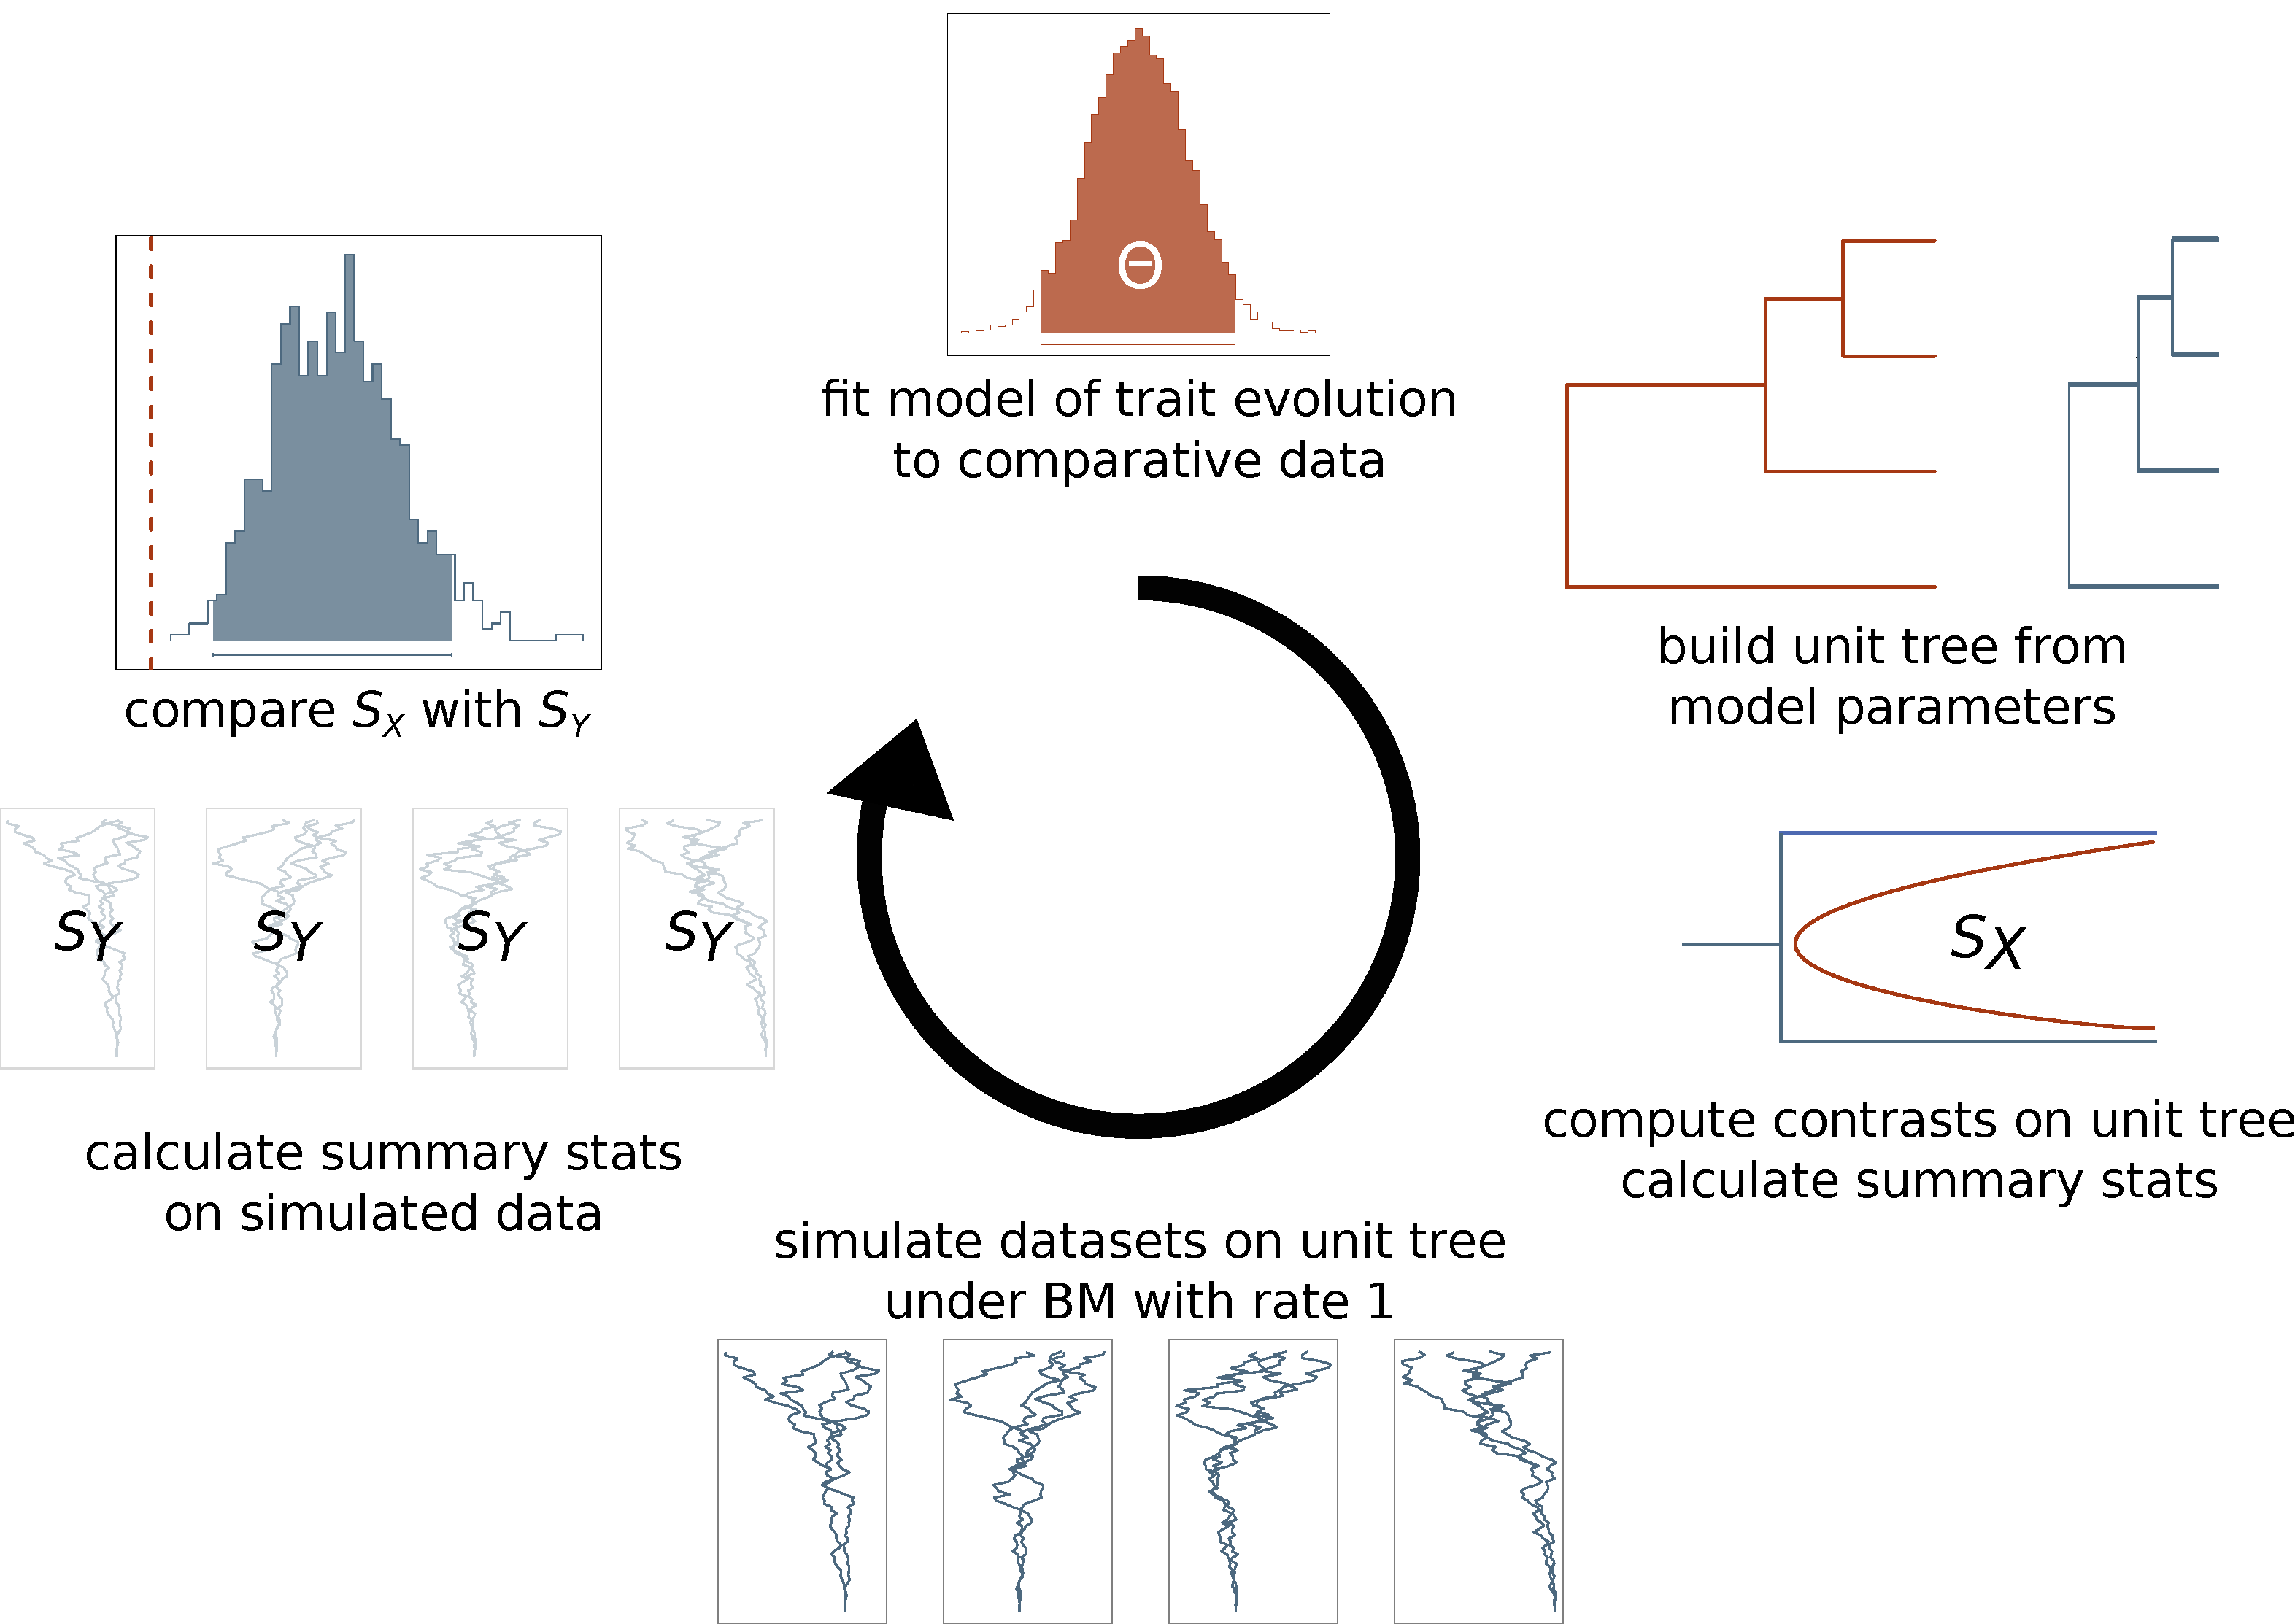
\includegraphics[scale=0.28]{figs/flowchart}
  \caption{Schematic diagram representing our approach for assessing model adequacy. 1) Fit a model of trait evolution to the data; 2) use the estimated model parameters to build a unit tree; 3) compute the contrasts from the data on the unit tree and calculate a set of summary statistics $\mathcal{S}_X$; 4) simulate a large number of datasets on the unit tree, using a BM model with $\sigma^2=$ 1; 5) calculate the summary statistics on the contrasts of each simulated dataset $\mathcal{S}_Y$; and 6) compare the observed and simulated summary statistics. If the observed summary statistic lies in the tails of the distribution of simulated summary statistics the model can be rejected as inadequate. The rotational circle in the center of the diagram indicates that assess model adequacy is an iterative process. If a model is rejected as inadequate, the next step is to propose a new model and repeat the procedure.}
  \label{fig:flowchart}
\end{figure}

\begin{figure}[p]
  \centering
  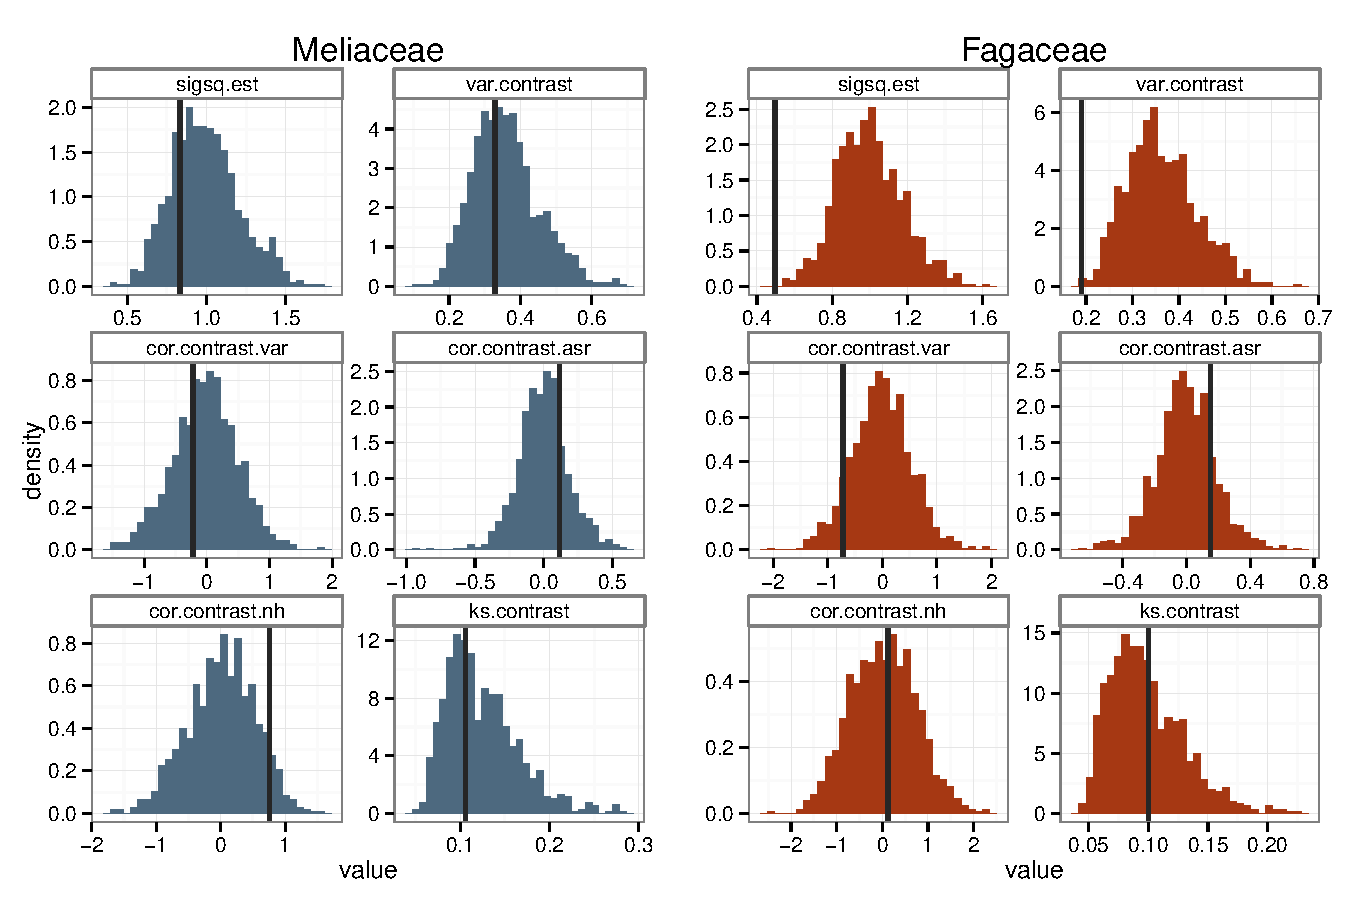
\includegraphics[scale=0.5]{figs/two-clade-example}
  \caption{Illustration of our approach to model adequacy. We fit three models (BM, OU, and EB) to seed mass data from two different tree families, the Meliaceae and the Fagaceae. In both cases, an OU model was strongly supported when fit with ML. The plotted distributions are the summary statistics ($M_{PIC}, V_{PIC}, S_{VAR}, S_{ANC}, S_{HGT}, D_{KS}$) calculated from the contrasts of the simulated data; the bars underneath the plots represent 95\% of the density. The dashed vertical lines are the values of the summary statistics calculated on the contrasts of the observed data. Using our summary statistics, an OU model appears to be an adequate model for the evolution of seed mass in the Meliaceae; for all of the summary statistics, the observed summary statistic lies in the middle of the distribution of simulated summary statistics. For the Fagaceae, the rate estimate $M_{PIC}$ from the observed data is much lower that the rate estimate calculated on the simulated datasets. We can therefore reject an OU model as inadequate for this group (see text for details).}
  \label{fig:two-clades}
\end{figure}

\begin{figure}[p]
  \centering
  \caption{Big fancy tree figure}
  \label{fig:angio-phylogeny}
\end{figure}

\begin{figure}[p]
  \centering
  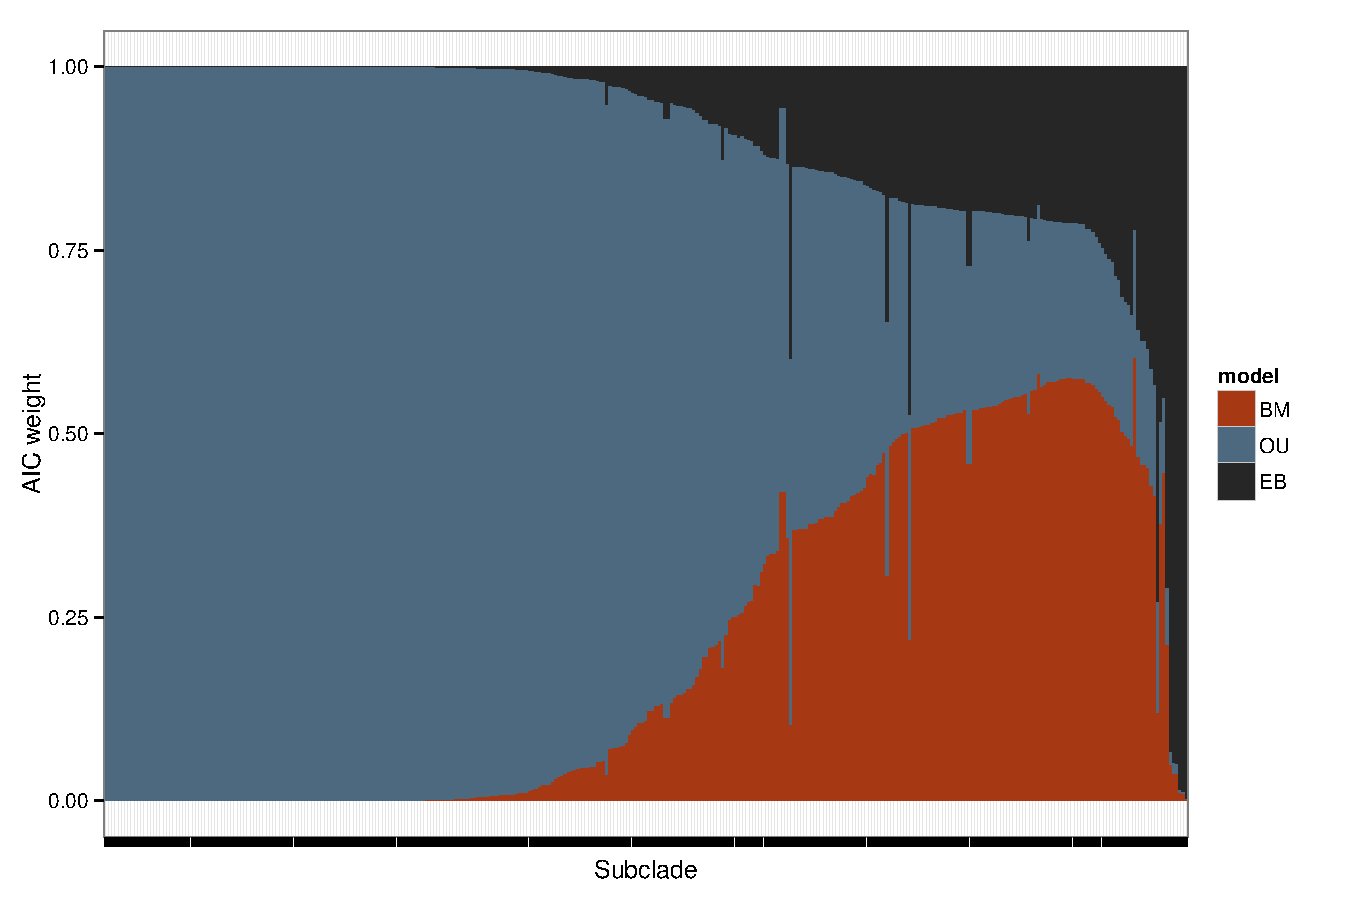
\includegraphics[angle=90, origin=c, scale=0.8]{figs/AIC-support}
  \caption{The relative support, as measured by AIC weight, for the three models used in our study (BM, OU, and EB) across all 337 datasets. An OU model is highly supported for a majority of the datasets.}
  \label{fig:aic-support}
\end{figure}

\begin{figure}[p]
  \centering
  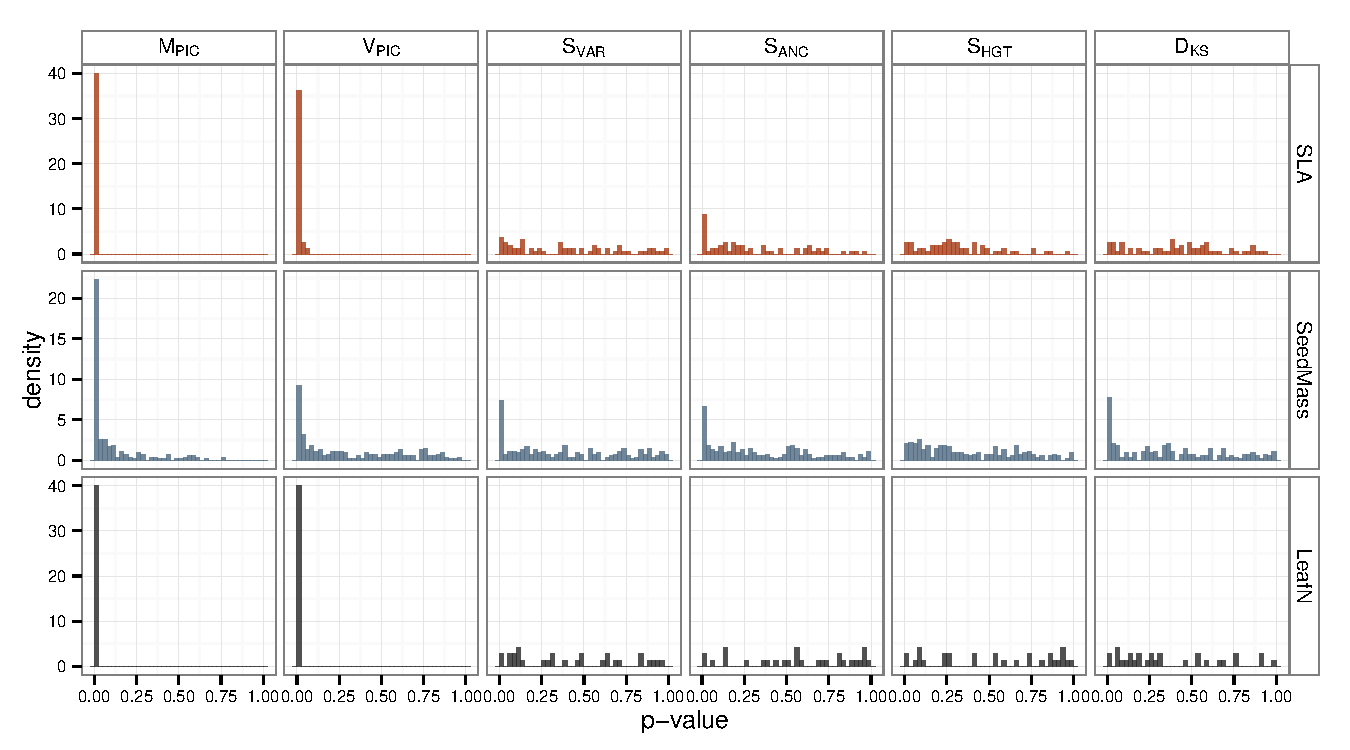
\includegraphics[angle=90, origin=c, scale=0.85]{figs/pvalue-hist-ML}
  \caption{The distribution of $p$--values for our six summary statistics over all 337 datasets in our study. This is from the results of fitting the models using ML; the $p$--values are those from applying our model adequacy approach to the best supported of the three models (as evaluated with AIC). For both the rate estimate $M_{PIC}$ and the coefficient of variation $V_{PIC}$, the vast majority of datasets would reject the best of the three models (at $p<$ 0.05).}
  \label{fig:pvalues}
\end{figure}

\begin{figure}[p]
  \centering
  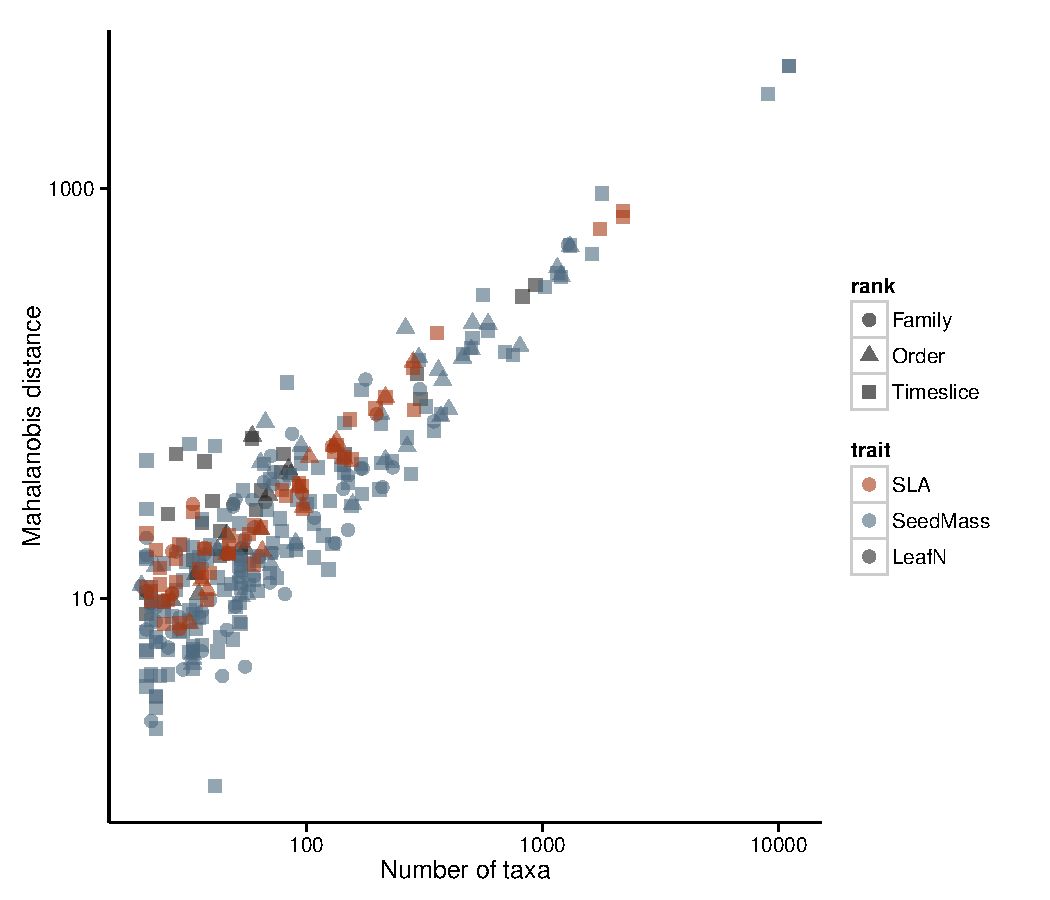
\includegraphics[scale=0.9]{figs/Size-adequacy-ML-bestonly}
  \caption{The relationship between clade size and a multivariate measure of model adequacy. The Mahalanobis distance is a scale--invariant metric that measures the distance between the observed and simulated summary statistics, taking into account the covariance between summary statistics. The greater the Mahalanobis distance, the worse the model captures variation in the data. There is a striking relationship between the two --- the larger the dataset, the worse the models performed (note the logarithmic scale). If the models were equally likely to be adequate at all scales, we would expect no relationship.}
  \label{fig:size-adequacy}
\end{figure}

\renewcommand\thefigure{Box\arabic{figure}}
\renewcommand\thetable{Box \arabic{table}}
\setcounter{figure}{0}    
\setcounter{table}{0} 

\begin{figure}[p]
  \centering
  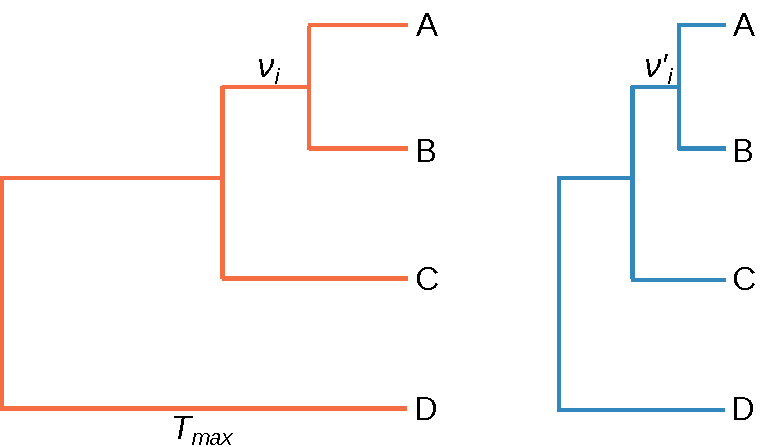
\includegraphics{figs/unit-tree}
  \caption{Illustration of creating a unit tree from model parameters. The original tree is in red. The unit tree constructed from an OU model with parameters $\sigma^2$ = 0.5 and $\alpha=$ 1 is in blue. The length of branch $i$, $\nu_i$ is rescaled to $v_i^\prime$ using Equation 3. Not only have the branch lengths changed relative to one another but the total tree depth $T$ has changed as well. While the tree on the left had branch lengths in units of time, the unit tree has branch lengths in units of (standardized) variance.}
  \label{fig:box1}
\end{figure}

\end{document}


